%%%%%%%%%%%%%%%%%%%%%%%%%%%%%%%%%%%%%%%%%%%%%%%%%%%%%%%%%%%%%%%%%%%%%%%%%%%%%%%%%%%%%%%%%%%%%%
%%%%%%%%%%%%%%%%%%%%%%%%%%%%%%%%%%%%%%%%%%%%%%%%%%%%%%%%%%%%%%%%%%%%%%%%%%%%%%%%%%%%%%%%%%%%%%
%%%%%%%%%%% GPU
%%%%%%%%%%%%%%%%%%%%%%%%%%%%%%%%%%%%%%%%%%%%%%%%%%%%%%%%%%%%%%%%%%%%%%%%%%%%%%%%%%%%%%%%%%%%%%
%%%%%%%%%%%%%%%%%%%%%%%%%%%%%%%%%%%%%%%%%%%%%%%%%%%%%%%%%%%%%%%%%%%%%%%%%%%%%%%%%%%%%%%%%%%%%%

% \cleardoublepage
\chapter{Equalizer Equations}
\label{chap:eq_eq}
This thesis examines that performance and GPU implementation of 5 equalizers.
While the performance and GPU implementation is interesting, this thesis makes no claim of theoretically expanding understanding of equalizers.
The data-aided equalizers studied in this thesis are:
\begin{itemize}
\item Zero-Forcing (ZF)
\item Minimum Mean Square Error (MMSE)
\item Constant Modulus Algorithm (CMA)
\item Frequency Domain Equalizer 1 (FDE1)
\item Frequency Domain Equalizer 2 (FDE2)
\end{itemize}
The ZF and MMSE equalizers are very similar in formulation though from different sources.
As you might tell from the names, FDE1 and FDE2 are also very similar with one subtle difference.
CMA isn't related to any other algorithm aside from being initialized by MMSE.

\section{Zero-Forcing and Minimum Mean Square Error Equalizers}
\label{sec:ZFnMMSE}
The ZF and MMSE equalizers are treated together here because they have many common features.
Both equalizers are found by solving linear equations
\begin{equation}
\mathbf{R}\mathbf{c} = \hat{\mathbf{h}}
\end{equation}
where $\mathbf{c}$ is a vector of desired equalizer coefficients
and $\mathbf{R}$ is an auto-correlation matrix of the channel estimate $\hat{\mathbf{h}}$.
It will be shown that the only difference between ZF and MMSE lies in the the auto-correlation matrix $\mathbf{R}$.

\subsection{Zero-Forcing}
\label{sec:zero-forcing}
The ZF equalizer is an FIR filter defined by the coefficients
\begin{equation}
\begin{matrix}
c_\text{ZF}(-L_1) & \cdots & c_\text{ZF}(0) & \cdots & c_\text{ZF}(L_2).
\end{matrix}
\end{equation}
The filter coefficients are the solution to the matrix vector equation \cite[eq. (311)]{PAQ-phase1}
\begin{equation}
\mathbf{c}_\text{ZF} = \big(\mathbf{H}^\dagger\mathbf{H}\big)^{-1} \mathbf{H}^\dagger \mathbf{u}_{n_0}
\label{eq:c_ZF_direct}
\end{equation}
where
\begin{equation}
\mathbf{c}_\text{ZF} = 
\begin{bmatrix}
c_\text{ZF}(-L_1) \\ \vdots \\ c_\text{ZF}(0) \\ \vdots \\ c_\text{ZF}(L_2)
\end{bmatrix},
\end{equation}
\begin{equation}
\mathbf{u}_{n_0} = \begin{bmatrix} 0 \\ \vdots \\ 0 \\ 1 \\ 0 \\ \vdots \\ 0 \end{bmatrix}
	\begin{matrix*}[l] \left. \vphantom{\begin{matrix} 0 \\ \vdots \\ 0 \end{matrix}} \right\}
		\text{$n_0-1$ zeros}
		\\ \\
		\left. \vphantom{\begin{matrix} 0 \\ \vdots \\ 0 \end{matrix}} \right\}
		\text{$N_1+N_2+L_1+L_2-n_0+1$ zeros}
		\end{matrix*},
		\label{eq:un0_ZF}
\end{equation}
where $n_0 = N_1+L_1+1$ and
\begin{equation} 
\mathbf{H} = 
		\begin{bmatrix}
		\hat{h}(-N_1)		&  				& 		 	&  					\\
		\hat{h}(-N_1+1) 	& \hat{h}(-N_1)	& 		 	&  					\\
		\vdots	 			& \vdots		& \ddots 	&  					\\
		\hat{h}(N_2)		& \hat{h}(N_2-1)&  			& \hat{h}(-N_1)  	\\
		 					& \hat{h}(N_2) 	&  			& \hat{h}(-N_1+1) 	\\
		 					&  	   			&  			& \vdots			\\
		 					&  	   			&  			& \hat{h}(N_2)		\\
	\end{bmatrix}.
\end{equation}

Equation \eqref{eq:c_ZF_direct} can be implemented directly but there are many optimization that greatly reduce computation.
The heaviest computation is the $\mathcal{O}(n^3)$ inverse operation followed by the $\mathcal{O}(n^2)$ matrix matrix multiplies.
Rather than performing a heavy inverse, multiplying $\mathbf{H}^\dagger \mathbf{H}$ on both sides of equation \eqref{eq:c_ZF_direct} results in
\begin{align}
\mathbf{H}^\dagger\mathbf{H} \mathbf{c}_\text{ZF} &= \mathbf{H}^\dagger \mathbf{u}_{n_0} \nonumber \\
\mathbf{R}_{\hat{h}} \mathbf{c}_\text{ZF} &= \hat{\mathbf{h}}_{n_0}
\label{eq:c_ZF_solve}
\end{align}
where
\begin{equation}
\mathbf{R}_{\hat{h}} = 
\mathbf{H}^\dagger \mathbf{H} = 
		\begin{bmatrix}
		r_{\hat{h}}(0)			& r^\ast_{\hat{h}}(1)	& \cdots 	& r^\ast_{\hat{h}}(L_{eq}-1)  	\\
		r_{\hat{h}}(1) 			& r_{\hat{h}}(0)		& \cdots 	& r^\ast_{\hat{h}}(L_{eq}-2)  	\\
		\vdots	 				& \vdots				& \ddots 	&  								\\
		r_{\hat{h}}(L_{eq}-1)	& r_{\hat{h}}(L_{eq}-2)	& \cdots	& r_{\hat{h}}(0)  			
	\end{bmatrix}
	\label{eq:R_h}
\end{equation}
is the auto-correlation matrix of the channel estimate $\hat{\mathbf{h}}$
and 
\begin{equation}
\hat{\mathbf{h}}_{n_0} = \mathbf{H}^\dagger \mathbf{u}_{n_0} = 
\begin{bmatrix} \hat{h}^\ast(L_1) \\ \vdots \\ \hat{h}^\ast(0) \\ \vdots \\ \hat{h}^\ast(-L_2)  \end{bmatrix}
\label{eq:h_no}
\end{equation}
is a vector with the time reversed and conjugated channel estimate $\hat{\mathbf{h}}$ centered at $n_0$.
The channel estimate auto-correlation sequence is
\begin{equation}
r_{\hat{h}}(k) = \sum_{n=-N_1}^{N_2} \hat{h}(n) \hat{h}^\ast(n-k).
\label{eq:sample_autocorrelation}
\end{equation}
Note that the auto-correlation matrix $\mathbf{R}_{\hat{h}}$ is comprised of 
\begin{equation}
\mathbf{r}_{\hat{h}} = 
\begin{bmatrix} r_{\hat{h}}(0) \\ \vdots \\ r_{\hat{h}}(L_{ch}) \\ r_{\hat{h}}(L_{ch}+1) \\ \vdots \\ r_{\hat{h}}(L_{eq}-1)\end{bmatrix} =
\begin{bmatrix} r_{\hat{h}}(0) \\ \vdots \\ r_{\hat{h}}(L_{ch}) \\ 0 \\ \vdots \\ 0  \end{bmatrix}.
\end{equation} 
Using $\mathbf{r}_{\hat{h}}$ eliminates the need for matrix matrix multiply of $\mathbf{H}^\dagger\mathbf{H}$.
Also, $r_{\hat{h}}(k)$ only has support on $-(L_{ch}-1) \leq k \leq L_{ch}-1$ making $\mathbf{R}_{\hat{h}}$ sparse or $\%63$ zeros. NEEDS CHECKING!!!!
The sparseness of $\mathbf{R}_{\hat{h}}$ can be leveraged to reduce computation drastically.

\subsection{MMSE Equalizer}
The MMSE equalizer is an FIR filter defined by the coefficients
\begin{equation}
\begin{matrix}
c_\text{MMSE}(-L_1) & \cdots & c_\text{MMSE}(0) & \cdots & c_\text{MMSE}(L_2).
\end{matrix}
\end{equation}
The filter coefficients are the solution to the matrix vector equation \cite[eq. (330) and (333)]{PAQ-phase1}
\begin{equation}
\mathbf{c}_{MMSE} = \big[ \mathbf{G}\mathbf{G}^\dagger + 2\hat{\sigma}^2_w\mathbf{I}_{L_1+L_2+1} \big]^{-1} \mathbf{g}^\dagger
\label{eq:c_MMSE_direct}
\end{equation}
where $\mathbf{I}_{L_1+L_2+1}$ is the $(L_1+L_2+1)\times(L_1+L_2+1)$ identity matrix,
$\hat{\sigma}^2_w$ is the estimated noise variance, $\mathbf{G}$ is the $(L_1+L_2+1)\times(N_1+N_2+L_1+L_2+1)$ matrix given by
\begin{equation}
\mathbf{G} = 
		\begin{bmatrix}
		\hat{h}(N_2)		& \cdots		& \hat{h}(-N_1) 	&  				  \\
							& \hat{h}(N_2)	& \cdots 			& \hat{h}(-N_1)	  \\
				 			& 				& \ddots 			&  				& \ddots	  \\
		 					&  	   			&  					& \hat{h}(N_2)	& \cdots	& \hat{h}(-N_1)	\\
	\end{bmatrix}
\end{equation}
and $\mathbf{g}^\dagger$ is the $(L_1+L_2+1)\times1$ vector given by
\begin{equation}
\mathbf{g}^\dagger = \hat{\mathbf{h}}_{n0} = \begin{bmatrix} \hat{h}^\ast(L_1) \\ \vdots \\ \hat{h}^\ast(0) \\ \vdots \\ \hat{h}^\ast(-L_2)  \end{bmatrix}.
%\begin{bmatrix} \hat{h}(L_1) \cdots \hat{h}(-L_2) \end{bmatrix}.
\label{eq:g_dagger_h_n0}
\end{equation}

Computing $\mathbf{c}_\text{MMSE}$ can be simplified by noticing that $\mathbf{g}^\dagger = \hat{\mathbf{h}}_{n_0}$, $\mathbf{G}\mathbf{G}^\dagger = \mathbf{R}_{\hat{h}}$ in Equation \eqref{eq:R_h}.
To further simplify MMSE, twice the estimated noise variance is added down the diagonal of the channel estimate auto-correlation matrix
\begin{equation}
\mathbf{R}_{\hat{h}w} = 
\mathbf{R}_{\hat{h}} + 2\hat{\sigma^2_w} \mathbf{I}_{L_1+L_2+1} = 
		\begin{bmatrix}
		r_{h}(0) + 2\hat{\sigma^2_w}	& r^\ast_{h}(1)							& \cdots 	& r^\ast_{h}(L_{eq}-1)  	\\
		r_{h}(1) 						& r_{h}(0) + 2\hat{\sigma^2_w}& \cdots 	& r^\ast_{h}(L_{eq}-2)  				\\
		\vdots	 						& \vdots								& \ddots 	&  							\\
		r_{h}(L_{eq}-1)					& r_{h}(L_{eq}-2)						& \cdots	& r_{h}(0) + 2\hat{\sigma^2_w}  			
	\end{bmatrix}.
	\label{eq:R_MMSE}
\end{equation}
By placing Equation \eqref{eq:R_MMSE} and \eqref{eq:g_dagger_h_n0} into \eqref{eq:c_MMSE_direct} results in
\begin{equation}
\mathbf{c}_\text{MMSE} = \mathbf{R}_{\hat{h}w}^{-1} \hat{\mathbf{h}}_{n_0}.
\end{equation}
Solving for the MMSE equalizer coefficients $\mathbf{c}_\text{MMSE}$ takes the form like the ZF equalizer coeffiencts in \eqref{eq:c_ZF_solve}
\begin{equation}
\mathbf{R}_{\hat{h}w}\mathbf{c}_\text{MMSE} = \hat{\mathbf{h}}_{n_0}.
\label{eq:c_MMSE_solve}
\end{equation}

The only difference between solving for the ZF and MMSE equalizer coefficients is $\mathbf{R}_{\hat{h}w}$ and $\mathbf{R}_{\hat{h}}$. 
The MMSE equalizer coefficients $\mathbf{c}_\text{MMSE}$ uses the noise variance estimate when building $\mathbf{R}_{\hat{h}w}$.
The sparseness of $\mathbf{R}_{\hat{h}w}$ can also be leveraged to reduce computation drastically because
$\mathbf{R}_{\hat{h}w}$ has the same sparse properties as $\mathbf{R}_{\hat{h}}$.

\section{The Constant Modulus Algorithm}
\label{sec:CMA}
The $b$th CMA equalizer is an FIR filter defined by the coefficients
\begin{equation}
\begin{matrix}
c_\text{CMA($b$)}(-L_1) & \cdots & c_\text{CMA($b$)}(0) & \cdots & c_\text{CMA($b$)}(L_2).
\end{matrix}
\end{equation}
The filter coefficients are calculated by a steepest decent algorithm 
\begin{equation}
\mathbf{c}_\text{CMA($b+1$)} = \mathbf{c}_\text{CMA($b$)}-\mu \nabla J
\label{eq:steepest}
\end{equation}
initialized by the MMSE equalizer coefficients
\begin{equation}
\mathbf{c}_\text{CMA($0$)} = \mathbf{c}_\text{MMSE}.
\end{equation}
The vector $\mathbf{J}$ is the cost function and $\nabla J$ is the cost function gradient \cite[eq. (352)]{PAQ-phase1}
\begin{equation}
	\nabla J = \frac{2}{L_{pkt}} \sum_{n=0}^{L_{pkt}-1}
	\left[ \vphantom{\displaystyle\sum}  y(n) y^\ast(n) - 1 \right]
	y(n)  \mathbf{r}^\ast(n).
\label{eq:DelJcma-approxr}
\end{equation}
where
\begin{equation}
\mathbf{r}(n) = \begin{bmatrix} r(n+L_1) \\ \vdots \\ r(n) \\ \vdots \\ r(n-L_2) \end{bmatrix}.
\end{equation}
This means $\nabla J$ is defined by
\begin{equation}
\nabla J = \begin{bmatrix} \nabla J(-L_1) \\ \vdots \\ \nabla J(0) \\ \vdots \\ \nabla J(L_2) \end{bmatrix}.
\end{equation}

A DSP engineer could implement the steepest decent algorithm by computing the cost function gradient directly.
The long summation for $\nabla J$ in \eqref{eq:DelJcma-approxr} does not map well to GPUs.
Later chapters will show how well convolution performs on GPUs.
The computation for $\nabla J$ can be massaged and re-expressed as convolution.

To begin messaging $\nabla J$, the term
\begin{equation}
z(n) = 	2\left[ \vphantom{\displaystyle\sum}  y(n) y^\ast(n) - 1 \right] y(n)
\end{equation} 
is defined to simplify the expression of $\nabla J$ to
\begin{equation}
	\nabla J = \frac{1}{L_{pkt}} \sum_{n=0}^{L_{pkt}-1}
	z(n)  \mathbf{r}^\ast(n).
\label{eq:DelJcma-midMassage}
\end{equation}
Expanding the expression of $\nabla J$ into vector form
\begin{multline}
\nabla J
	= 
	\frac{z(0)}{L_{pkt}}
		\begin{bmatrix} r^\ast(L_1) \\ \vdots \\ r^\ast(0) \\ \vdots \\ r^\ast(L_2) \end{bmatrix} +
	\frac{z(1)}{L_{pkt}}
		\begin{bmatrix} r^\ast(1+L_1) \\ \vdots \\ r^\ast(1) \\ \vdots \\ r^\ast(1-L_2) \end{bmatrix} + \cdots
	\frac{z(L_{pkt}-1)}{L_{pkt}}
		\begin{bmatrix} r^\ast(L_{pkt}-1+L_1) \\ \vdots \\ r^\ast(L_{pkt}-1) \\ \vdots \\ r^\ast(L_{pkt}-1-L_2) \end{bmatrix}
\label{eq:delJ_writeoutr}
\end{multline}
shows a pattern in $z(n)$ and $\mathbf{r}(n)$.
The $k$th value of $\nabla J$ is
\begin{equation}
\nabla J(k) = \frac{1}{L_{pkt}} \sum^{L_{pkt}-1}_{m=0}  z(m) r^\ast(m-k), \quad -L_1 \leq k \leq L_2.
\label{eq:delJ_direct_way}
\end{equation}
The summation almost looks like a convolution accept the conjugate on the element $r(n)$.
To put the summation into the familiar convolution form, define
\begin{equation}
\rho(n) = r^\ast(n).
\end{equation}
Now
\begin{equation}
\nabla J(k) = \frac{1}{L_{pkt}} \sum^{L_{pkt}-1}_{m=0}  z(m) \rho(k-m).
\label{eq:CMA_delJ_rice_reformed}
\end{equation}

Note that $z(n)$ has support on $0 \leq n \leq \Lpkt-1$ and 
$\rho(n)$ has support on $-\Lpkt+1 \leq n \leq 0$, 
the long result of the convolution sum $b(n)$ has support on $-\Lpkt+1 \leq n \leq \Lpkt-1$.
Putting all the pieces together, we have
\begin{align}
b(n) &= \sum^{L_{pkt}-1}_{m=0} z(m) \rho(n-m) \nonumber \\
	 &= \sum^{L_{pkt}-1}_{m=0} z(m) r^\ast(m-n)
	 \label{eq:CMA_conv_z_rho}
\end{align}
Comparing Equation \eqref{eq:CMA_delJ_rice_reformed} and \eqref{eq:CMA_conv_z_rho} shows that 
\begin{equation}
\nabla J(k) = \frac{1}{L_{pkt}} b(k), \quad -L_1 \leq k \leq L_2.
\label{eq:CMA_delJ_donzo}
\end{equation}
The values of interest are shown in Figure \ref{fig:convolutionFigureRice}.
\begin{figure}
	\centering\includegraphics[width=10in/100*55]{figures/eq_equations/convolutionFigureRice.pdf}
	\label{fig:convolutionFigureRice}
	\caption{Diagram showing the relationships between $z(n)$, $\rho(n)$ and $b(n)$.}
\end{figure}

This suggest the following matlab code for computing computing the gradient vector $\nabla J$ and implementing CMA.
\begin{table}[h]
\caption{CMA}
\label{code:CMA}
\singlespacing
{\footnotesize
\begin{verbatim}
 1 c_CMA = c_MMSE;
 2 for i = 1:its
 3 yy = conv(r,c_CMAb);
 4 y = yy(L1+1:end-L2); % trim yy
 5 z = 2*(y.*conj(y)-1).*y;
 6 Z = fft(z,Nfft);
 7 R = fft(conj(r(end:-1:1)),Nfft)
 8 b = ifft(Z.*R);
 9 delJ = b(Lpkt-L1:Lpkt+L2);
10 c_CMAb1 = c_CMAb -mu*delJ;
11 c_CMAb = c_CMAb1;
12 end
13 yy = conv(r,c_CMA);
14 y = yy(L1+1:end-L2); % trim yy
\end{verbatim}
}
\end{table}
\doublespacing

\clearpage
\section{The Frequency Domain Equalizers}
\label{sec:FDE}
Frequency Domain Equalizer One (FDE1) and Frequency Domain Equalizer Two (FDE2) are very similar and have the same structure.
FDE1 and FDE2 are adapted from Williams' and Saquib's Frequency Domain Equalizers \cite[eq. (11) and (12)]{williams2013linear}.

\subsection{Frequency Domain Equalizer One}
FDE1 is the MMSE or Wiener filter applied in the frequency domain from Williams' and Saquib's paper \cite[eq. (11)]{williams2013linear}
\begin{equation}
C_\text{FDE1}(e^{j\omega_k}) = \frac{\hat{H}^\ast(e^{j\omega_k})}  {|\hat{H}(e^{j\omega_k})|^2  +  \frac{1}{\hat{\sigma}^2_w}} \quad
\text{where} \;
\omega_k = \frac{2\pi}{L} \;
\text{for} \;
k=0,1,\cdots,L-1.
\label{eq:FDE1}
\end{equation}
The term $C_\text{FDE1}(e^{j\omega_k})$ is FDE1s frequency response at $\omega_k$.
The term $\hat{H}(e^{j\omega_k})$ is the channel estimate frequency response at $\omega_k$.
The term $\hat{\sigma}^2$ is the noise variance estimate, this term is completely independent of frequency because the noise is assumed to be spectrally flat or white.

Equation \eqref{eq:FDE1} is straight forward to implement in GPUs.
FDE1 is extremely fast and computationally efficient.

\subsection{Frequency Domain Equalizer Two}
FDE2 is also the MMSE or Wiener filter applied in the frequency domain but knowledge of the SOQPSK-TG spectrum is leveraged \cite[eq. (12)]{williams2013linear}.
The frequency respoonse of FDE2 is
\begin{equation}
C_\text{FDE2}(e^{j\omega_k}) = \frac{\hat{H}^\ast(e^{j\omega_k})}  {|\hat{H}(e^{j\omega_k})|^2  +  \frac{\Psi(e^{j\omega_k})}{\hat{\sigma}^2_w}} \quad
\text{where} \;
\omega_k = \frac{2\pi}{L} \;
\text{for} \;
k=0,1,\cdots,L-1
\label{eq:FDE2}
\end{equation}
where $\Psi(e^{j\omega_k})$ is show in Figure \ref{fig:SOQPSK_spectrum}.
The term $\Psi(e^{j\omega_k})$ eliminates out of band multipath that may be challenging to estimate and over come.
\begin{figure}
	\centering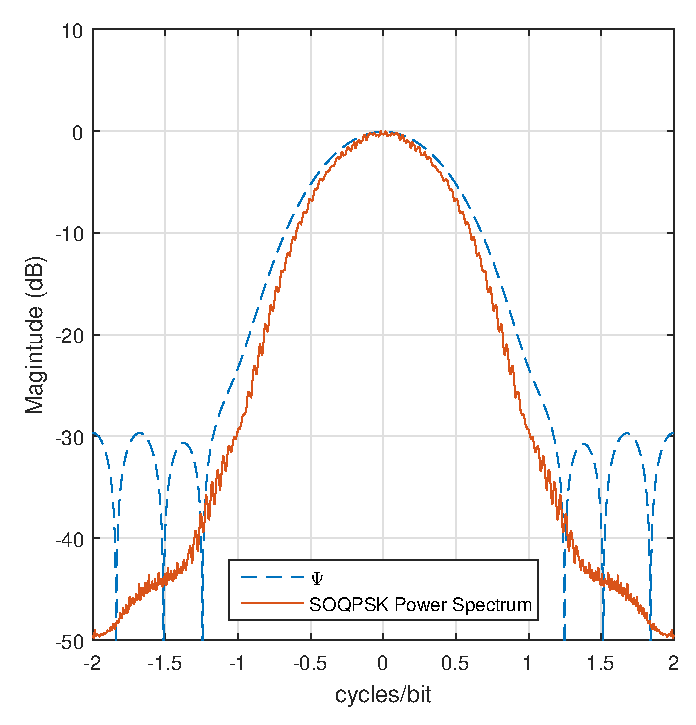
\includegraphics[width=5in]{figures/eq_equations/FDE2_spectrum_PSI.eps}
	\label{fig:SOQPSK_spectrum}
	\caption{I need help on this one!!!! }
\end{figure}
